\documentclass[tikz]{standalone}
\usetikzlibrary{shapes,arrows.meta}
\begin{document}
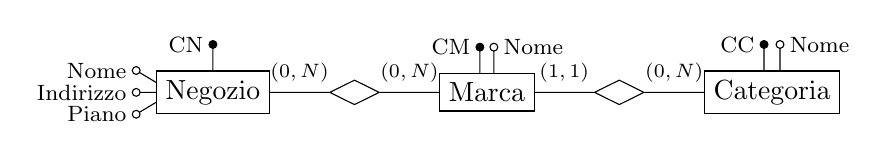
\begin{tikzpicture}
    \draw

    %%* Attributi:
    %%  node[draw, circle, inner sep=1pt, fill=black]{}node[right]{\footnotesize A}
    %%? Distanza orizzontale: E -(0.25,0.x)- A
    %%? Distanza verticale: E -(0,x * 0.22)- A

    %%* Cardinalità:
    %%  node[below right]{\scriptsize $(0,N)$}
    %%  node[above right]{\scriptsize $(0,N)$}
    %%  node[midway, above]{\scriptsize $(0,N)$}

    %%* Relazione:
    %%  node[draw, diamond, shape aspect=2, inner sep=3pt, anchor=90](r1){}
    %%  node[draw, diamond, shape aspect=2, inner sep=0.2pt, anchor=180](r2){R2}

    %%* Entità:
    %%  node[draw, rectangle, anchor=90](e1){}
    %%? Distanza verticale: E -(0.3)- R -(0.3) E
    %%? Distanza orizzontale: E -(0.75)- R -(0.75)- E

    %%* Negozio
    (0,0)node[draw, rectangle, anchor=90](e1){Negozio}
    (e1.0)--++(0.75,0)node[midway, above]{\scriptsize $(0,N)$}node[draw, diamond, shape aspect=2, inner sep=3pt, anchor=180](r1){}

    (e1.170)--++(-0.25,0.15) node[draw, circle, inner sep=1pt, fill=white]{}node[left]{\footnotesize Nome}
    (e1.180)--++(-0.25,0) node[draw, circle, inner sep=1pt, fill=white]{}node[left]{\footnotesize Indirizzo}
    (e1.190)--++(-0.25,-0.15)node[draw, circle, inner sep=1pt, fill=white]{}node[left]{\footnotesize Piano}
    (e1.90)--++(0,0.33)node[draw, circle, inner sep=1pt, fill=black]{}node[left]{\footnotesize CN}

    %%* Marca
    (r1.0)--++(0.75,0)node[midway, above]{\scriptsize $(0,N)$}node[draw, rectangle, anchor=180](e2){Marca}
    (e2.0)--++(0.75,0)node[midway, above]{\scriptsize $(1,1)$}node[draw, diamond, shape aspect=2, inner sep=3pt, anchor=180](r2){}

    (e2.110)--++(0,0.33)node[draw, circle, inner sep=1pt, fill=black]{}node[left]{\footnotesize CM}
    (e2.70)--++(0,0.33)node[draw, circle, inner sep=1pt, fill=white]{}node[right]{\footnotesize Nome}

    %%* Categoria
    (r2.0)--++(0.75,0)node[midway, above]{\scriptsize $(0,N)$}node[draw, rectangle, anchor=180](e3){Categoria}

    (e3.110)--++(0,0.33)node[draw, circle, inner sep=1pt, fill=black]{}node[left]{\footnotesize CC}
    (e3.70)--++(0,0.33)node[draw, circle, inner sep=1pt, fill=white]{}node[right]{\footnotesize Nome}
    
    ;
\end{tikzpicture}
\end{document}